\documentclass[11pt,letterpaper]{article}
\usepackage[T1]{fontenc}
\usepackage[utf8]{inputenc}
\usepackage{lmodern,microtype,amsmath,amssymb,amsthm,mathtools,booktabs,graphicx}
\usepackage[margin=0.94in,top=0.9in,bottom=0.9in]{geometry}
\usepackage{xcolor,fancyhdr}
\definecolor{inkblue}{HTML}{153F55}
\usepackage[colorlinks=true,linkcolor=inkblue,citecolor=inkblue,urlcolor=inkblue,bookmarksnumbered=true]{hyperref}
\hypersetup{pdftitle={Reconstructing complete multipartite graphs from Ehrhart polynomials},pdfauthor={OpenAI}}
\newtheorem{theorem}{Theorem}[section]
\newtheorem{lemma}[theorem]{Lemma}
\newtheorem{proposition}[theorem]{Proposition}
\newtheorem{corollary}[theorem]{Corollary}
\theoremstyle{remark}\newtheorem{remark}[theorem]{Remark}
\pagestyle{fancy}\fancyhf{}\fancyhead[L]{\small\itshape Multipartite Ehrhart polynomials}
\fancyhead[R]{\small November 2026}\fancyfoot[C]{\thepage}
\setlength{\headheight}{14pt}
\setlength{\parskip}{2pt}
\setlength{\emergencystretch}{2em}
\raggedbottom
\begin{document}
\thispagestyle{plain}
\begin{center}
{\LARGE\bfseries Reconstructing complete multipartite graphs\\[4pt] from Ehrhart polynomials\par}
\vspace{0.5em}
{\large Exact coefficients, interlacing, and the square-root threshold for zeros\par}
\vspace{0.7em}
{\small Research manuscript \enspace$\cdot$\enspace 27 November 2026}
\end{center}

\begin{abstract}
The Ehrhart polynomial of the symmetric edge polytope of a connected complete
multipartite graph determines the graph. We prove this by counting subsets
of $v-1$ vertices obtained by identifying a pair from different parts.
The formula gives nonnegative gamma coefficients and exact cross-degree
$\min(\lfloor(v-1)/2\rfloor,v-1-b)$, where $b$ is the largest part.
It resolves the cross-degree question in K\"olbl's Conjecture~4.8 and
gives strict interlacing for $K_{1^k,n}$ and $K_{1^{k+1},n}$ for
$1\le k\le20$ and all $n\ge1$.

For $K_{d+1}$ with a matching deleted, the possible finite limits of Ehrhart
zeros fill precisely $-1\le\Re s\le0$. We determine the counts on the
three limiting lines for a matching of order $d^\alpha$, $1/2<\alpha\le1$.
At the scale $M\sim c\sqrt d$ the sharp constant for bounded-region
stability over both parities is $c=\sqrt{8/\pi}$. The numerator of the
Ehrhart series loses real-rootedness at a different threshold, of order
$d^{3/4}$. A maximum matching yields asymptotically
$(\sqrt{2}/\pi)\sqrt{d\log d}$ nonreal numerator zeros.
The arguments are independent of Dirichlet GRH.
\end{abstract}

\section{The conjectures and the source of the method}
An Ehrhart polynomial records the number of lattice points in every
nonnegative integral dilation of a lattice polytope. Here the polytope
encodes the edges of a graph by the vectors $\pm(e_i-e_j)$. Its Ehrhart
polynomial has a reflection symmetry about the line $\Re s=-1/2$.
Higashitani, Kummer and Micha\l ek asked whether every zero lies on that
line for complete multipartite graphs~\cite[Conj.~4.10]{hkm}. Davis's
example with six parts of size two has four zeros off it~\cite{davis}.
How far can such zeros move when the graph differs from a complete
graph in only a few edges? Corollary~\ref{cor:strip} and
Theorem~\ref{thm:critical} give global and local answers.

The complete bipartite numerator and its real-rootedness are due to
Higashitani, Jochemko and Micha\l ek~\cite{hjm}. K\"olbl obtained a
tripartite numerator formula, several interlacings, and a two-part
question about cross-degree and split graphs~\cite{kolbl}. Ohsugi and
Tsuchiya's suspension theorem~\cite{ot} supplies the enumerative input
for our coefficient formula. Ferroni has exhibited symmetric edge polytopes of
other graphs with negative gamma coefficients~\cite{ferroni}.

The starting point in ProveIt is the graph section of its synthesis of
194 reports~\cite{repo}. Its complete-bipartite lattice membership test,
cross-polytope expansion, and positive Bezoutian certify canonical-line
zeros through fixed part sizes. We apply the multipartite membership
test to count the loss from each individual part. For interlacing we use
the repository's Bezoutian method on a different family, with one part
of arbitrary size and several singleton parts. For deletions, the same
expansion collapses to one correction term, for which singularity analysis
gives the zero law. The source theorem on Dirichlet $L$-functions
enters the repository's arithmetic sections. The graph argument can be
verified from the geometric and analytic inputs given here.

\section{The gamma vector of a complete multipartite graph}\label{sec:gamma}

Let $G=K_{a_1,\ldots,a_r}$ with $r\ge2$ nonempty parts $A_i$,
$v=\sum_i a_i$ vertices and $d=v-1$. Its symmetric edge polytope is
\[
 P_G=\operatorname{conv}\{\pm(e_u-e_w):uw\in E(G)\}
 \quad\text{in the lattice}\quad
 \{x\in\mathbb Z^v:\textstyle\sum_i x_i=0\}.
\]
The dimension is $d$ because the edge differences of a spanning tree span
the zero-sum hyperplane. Write $E_G(k)=|kP_G\cap\mathbb Z^v|$.
The Ehrhart numerator $h^*_G$ and its gamma coefficients are specified by
\[
  \sum_{k\ge0} E_G(k)t^k=\frac{h^*_G(t)}{(1-t)^{d+1}},\qquad
  h^*_G(t)=\sum_{0\le j\le d/2}\gamma_j(G)t^j(1+t)^{d-2j}.
\]
The second expansion follows here from the proof below. The largest index
with $\gamma_j\ne0$ is the \emph{cross-degree} of $E_G$ in
K\"olbl's terminology~\cite[Prop.~4.3]{kolbl}.

\begin{theorem}\label{thm:gamma}
Identify one vertex in each of two distinct parts with each other to form
a set $W$ of $d$ elements. Denote the images of the parts by $B_i$.
Then
\begin{equation}\label{eq:subset-gamma}
 \gamma_j(G)=\binom{2j}{j}\,
 \#\{T\subseteq W: |T|=2j,\ |T\cap B_i|\le j\text{ for every }i\}.
\end{equation}
In particular, all gamma coefficients are nonnegative. For
$0\le j\le\lfloor d/2\rfloor$ they satisfy the closed formula
\begin{equation}\label{eq:multipartite-gamma}
 \frac{\gamma_j(G)}{\binom{2j}{j}}
  =\binom{d}{2j}-
    \sum_{i=1}^r\sum_{\ell=j+1}^{2j}
       \binom{a_i}{\ell}\binom{d-a_i}{2j-\ell},
\end{equation}
where out-of-range binomial coefficients are zero.
\end{theorem}

\subsection{Lattice points and the loss from a single part}
For an integer vector $x$ of coordinate sum zero, let $p_i$ and $n_i$
denote the sums of its positive entries and the absolute values of its
negative entries in $A_i$. Put $q=\sum_i p_i=\sum_i n_i$.

\begin{lemma}\label{lem:gauge}
For integral $k\ge0$, membership $x\in kP_G$ is equivalent to
$q\le k$ and $p_i+n_i\le k$ for all $i$.
\end{lemma}
\begin{proof}
Each signed edge has total positive mass one and has at most one endpoint
in any one part. Convexity and the triangle inequality give necessity.
For sufficiency, view $x$ as a transportation problem with $q$ units each
of supply and demand. Direct transport across different parts can route
all units when $p_i+n_i\le q$ for every $i$. Indeed, treat each unit as a
distinct vertex of a bipartite graph of supply and demand. A set of
supplies in one part has access to $q-n_i\ge p_i$ demands. A set of
supplies meeting two parts has access to every demand. Hall's theorem
gives a perfect matching.

Otherwise exactly one part, say $h$, has $p_h+n_h=q+\delta$ with
$\delta>0$, since the sum of all $p_i+n_i$ equals $2q$. Pair $\delta$
supplies and demands in that part, routing each through any vertex in
another part. This is possible since $\delta\le\min(p_h,n_h)$.
The remaining total mass is $q-\delta$ on each side. Part $h$ holds
$q-\delta$ residual endpoints, and the other parts combined also hold
$q-\delta$. Hall's test now supplies a direct matching of the remaining
units. The total number of signed edges used is $q+\delta\le k$.
Since $0\in P_G$, this exhibits $x\in kP_G$.
\end{proof}

This criterion also follows from the known facet descriptions and is
the multipartite lattice-membership criterion used by Davis~\cite{davis}.
Its role here is to make the losses from different parts additive.
Let $G_i$ be the graph formed by deleting just the edges within $A_i$
from $K_v$, so all other vertices are singleton parts. In $kP_{K_v}$ the
sole bound is $q\le k$. A vector can violate $p_i+n_i\le k$ for at most
one $i$, since its total absolute mass is $2q\le2k$. Thus
\begin{equation}\label{eq:additive-defects}
 E_G=E_{K_v}-\sum_{i=1}^r(E_{K_v}-E_{G_i}).
\end{equation}
This identity at all nonnegative integers is also a polynomial identity.
Taking Ehrhart numerators is linear at the fixed dimension $d$.

\subsection{Balanced subsets for one part}
For a connected graph $F$ on a set $W_0$ of $d$ vertices, its suspension
$\widehat F$ adds a new vertex adjacent to every old vertex.
The cut formula of Ohsugi and Tsuchiya
\cite[Thm.~3.1 and Prop.~4.1]{ot} gives
\[
 \gamma_j(\widehat F)=
 \frac{4^j}{2^d}\sum_{S\subseteq W_0}
 \#\{T\subseteq W_0: |T|=2j,\ F[S,W_0\setminus S][T]
     \text{ has a perfect matching}\}.
\]
Here the graph inside the count retains only the edges crossing the
displayed cut, then restricts to $T$. The cut average is over all
ordered sides $S$; this counts complementary choices twice.
For a fixed ordered pair of disjoint $j$-subsets $U,V$, let $T=U\cup V$.
Exactly $2^{d-2j}$ cuts restrict to $U$ on $T$, with $V$ on the other
side. Consequently $\gamma_j(\widehat F)$ counts the ordered pairs
$(U,V)$ for which the bipartite edges of $F$ between $U$ and $V$ admit a
perfect matching. This counts each admissible pair once, irrespective of
the number of its perfect matchings.

The same ordered-pair description holds for an edgeless $F$: its
suspension is a star, whose incident edge differences are a lattice basis,
so its polytope is the cross-polytope with numerator $(1+t)^d$.

In $G_i$ take the suspension vertex outside $A_i$. The graph $F$ consists
of a complete graph on $d$ vertices with the edges within $A_i$ deleted. It is connected whenever an old vertex
outside $A_i$ remains, and edgeless otherwise.
On $U\cup V$, the sole possible obstruction to a perfect matching is
$|U\cap A_i|>|V\setminus A_i|$. Indeed, any subset of $U$ meeting
the complement of $A_i$ sees all of $V$, and a nonempty subset contained
in $A_i$ sees all of $V\setminus A_i$. Thus the admissibility condition
is exactly $|(U\cup V)\cap A_i|\le j$. Each such union admits
$\binom{2j}{j}$ choices of ordered sides. The same cut formula for
the complete graph counts all $2j$-element unions.
Substituting the resulting coefficients in \eqref{eq:additive-defects}
gives \eqref{eq:multipartite-gamma}, since the defect of part $i$
counts the unions with more than $j$ points in that part.

To prove \eqref{eq:subset-gamma}, take the common set $W$ obtained by
identification as in the theorem. Every $B_i$ has size $a_i$, and any two
distinct $B_i$ intersect in at most one point. If a $2j$-element set
violated two bounds, it would contain at least $2j+2-1$ points. Hence
the forbidden families are disjoint. Counting their complement gives
exactly the right side of \eqref{eq:multipartite-gamma}.
This completes the proof of Theorem~\ref{thm:gamma}.

\section{Exact cross-degree and the formulation of K\"olbl's question}
\label{sec:cross-degree}

\begin{theorem}\label{thm:crossdegree}
Put $b=\max_i a_i$ and $s=v-b$. The cross-degree of the complete
multipartite Ehrhart polynomial is
\begin{equation}\label{eq:degree}
 m=\min\{\lfloor(v-1)/2\rfloor,\ s-1\}.
\end{equation}
In fact $\gamma_j>0$ for every $0\le j\le m$.
\end{theorem}

\begin{proof}
We have $2j\le d$. The set $W$ contains just $d-b=s-1$ points outside
the largest $B_i$. A permitted $2j$-set needs at least $j$ outside that
part, so $j\le s-1$.

If $b<v/2$, set $j=\lfloor d/2\rfloor$. All parts have size at most $j$,
and every $2j$-set is permitted. Suppose next that $b\ge v/2$ and put
$j=s-1$. If there are at least three parts, each of the other parts has
size at most $s-1$. Choose all $s-1$ points outside a largest $B_i$ and
any $s-1$ points inside it. This attains the bound. With two parts of
sizes $a,b$, their two images intersect in a single point. A permitted
$2j$-set must avoid that point (the two intersection counts sum to at most
$2j$) and must take exactly $j$ of the $a-1$ and $b-1$ remaining points
on the two sides. In particular $j=\min(a,b)-1$ is attained; this also
recovers the complete bipartite formula of Higashitani, Jochemko and
Micha\l ek~\cite[Thm.~4.1]{hjm}.

Finally, from any permitted $2j$-set with $j\ge2$ one obtains a
permitted $(2j-2)$-set by removing two points that meet every part
containing exactly $j$ selected points. There are at most two such parts,
because the total of the intersection counts is at most $2j+1<3j$.
Choose one point from each if there are two (distinct choices are
possible since each contains $j\ge2$ points), or fill the two removals
arbitrarily after meeting a unique saturated part. When $j=1$ the empty
set suffices. This proves positivity at every smaller index.
\end{proof}

K\"olbl's Conjecture~4.8~\cite{kolbl} introduces
$a_1\le\cdots\le a_k\le n$, then prints $K_{a_1,\ldots,a_k}$ and the
bounds $\lfloor(\sum_i a_i)/2\rfloor\le m+1\le\sum_i a_i$.
On that literal reading the lower bound fails already at $K_{1,3}$,
where $m=0$ and $\lfloor4/2\rfloor=2$. If the unused $n$ designates
one further largest part, write $s=\sum_i a_i$. Formula~\eqref{eq:degree}
then gives
\[
  m+1=\min\{\lceil(s+n)/2\rceil,\ s\},
\]
which implies both displayed inequalities for $K_{a_1,\ldots,a_k,n}$ and
gives equality in the upper bound whenever $n\ge s-1$. The theorem
covers both graph conventions explicitly. The interlacing question for
$K_{1^k,n}$ and $K_{1^{k+1},n}$ concerns Ehrhart zeros and is a separate
part of the conjecture.

\section{Recovering all part sizes}\label{sec:inverse}
A consequence of the closed formula is an inverse theorem. For example,
$K_{1,4,4}$ and $K_{2,2,5}$ have the same dimension and the same number
of edges. The coefficient $\gamma_2$ distinguishes them.

\begin{theorem}[Reconstruction]\label{thm:inverse}
Among connected complete multipartite graphs on at least two vertices,
the Ehrhart polynomial of the symmetric edge polytope determines the graph
up to isomorphism. The multiset of part sizes can be recovered by integer
arithmetic.
\end{theorem}
\begin{proof}
The degree gives $d$, hence $v=d+1$. Compute the gamma vector from the
Ehrhart series, and put $h=\lfloor d/2\rfloor$. Write
\[
 D_j=\binom d{2j}-\gamma_j/\binom{2j}{j},\qquad
 L_j(a)=\sum_{\ell=j+1}^{2j}\binom a\ell\binom{d-a}{2j-\ell}.
\]
If the cross-degree $m<h$, Theorem~\ref{thm:crossdegree} gives the
largest part $b=d-m$. It exceeds $v/2$, so it occurs once.
Record it and subtract $L_j(b)$ from each $D_j$.
All remaining parts are at most $h+1$. The same bound holds for every
part when $m=h$, since then $b\le d-h$.

For $j=h,h-1,\ldots,1$, the remaining parts now have size at most $j+1$.
The value $L_j(a)$ vanishes at every $a\le j$, while
\[
 L_j(j+1)=\binom{d-j-1}{j-1}>0 .
\]
Divide the residual $D_j$ by this number to obtain the multiplicity of
$j+1$, then subtract its contributions from the remaining equations.
The total $d+1$ determines the number of singleton parts. The algorithm
works also for $d=1$, when only this last step is needed.
\end{proof}
Since $E_G(0)=1$, the complex zero multiset with multiplicities also
determines $E_G$ and hence $G$ in this class. At order nine the two
graphs above have respectively $\gamma_2=216$ and $\gamma_2=210$.

\section{Strict interlacing for split graphs}\label{sec:interlacing}

Write $E_{k,n}$ in this section for the Ehrhart polynomial of the graph
$K_{1^k,n}$, with $k$ singleton parts and one part of size $n$.
K\"olbl's interlacing conjecture asks what happens when one adds a
singleton, keeping $n$ fixed. His Theorem~3.3(a,d) gives the first two
steps~\cite{kolbl}. The following theorem has no upper bound on $n$.

\begin{theorem}\label{thm:split}
For $1\le k\le20$ and every positive integer $n$, the zeros of
$E_{k,n}$ and $E_{k+1,n}$ are simple, have real part $-1/2$, and strictly
interlace when ordered by imaginary part. In particular the simple-root
canonical-line property holds through $21$ singleton parts.
\end{theorem}

\begin{proof}
Let $r=k-1$, $d=n+r$. The formula of Theorem~\ref{thm:gamma}
specializes to
\[
 g_j=\binom{2j}{j}\sum_{\ell=0}^j
           \binom n\ell\binom r{2j-\ell}\qquad (0\le j\le r).
\]
Only the $n$-part can contain more than half of a set of size $2j$,
for $j\ge1$. We set $g_j=0$ for $2j>d$, as the formula already does.
Let $C_m$ be the cross-polytope Ehrhart polynomial and put
\[
 Q_m(y)=m!\,i^{-m}C_m((iy-1)/2).
\]
Then $Q_0=1$, $Q_1=y$ and
$Q_{m+1}=yQ_m-m^2Q_{m-1}$. This recurrence also follows by
differentiating the generating function
$\sum_{m\ge0}C_m(x)u^m=(1+u)^x/(1-u)^{x+1}$.
The gamma expansion, the Ehrhart series
$(1+t)^m/(1-t)^{m+1}$ of $C_m$, and
$4t=(1+t)^2-(1-t)^2$ give
\[
 R_{r,n}(y)=4^r d!\,i^{-d}E_{k,n}((iy-1)/2)
       =\sum_{0\le h\le\min(r,\lfloor d/2\rfloor)}
           (d)_{2h}\left(\sum_{j=h}^r 4^{r-j}g_j\binom jh\right)Q_{d-2h}(y).
\]
Here $(d)_a=d(d-1)\cdots(d-a+1)$. The leading coefficient is positive.

For $n\ge r+2$, apply the three-term recurrence in both directions to
write
\[
 R_{r,n}=A Q_n-B Q_{n-1},\qquad R_{r+1,n}=C Q_n-D Q_{n-1}.
\]
This expresses both polynomials using the pair $Q_n,Q_{n-1}$, as in the
repository's graph-tower section. In the first pair the degrees in $y$ are
at most $r,r-1$, respectively, and the respective parities are those of
$r,r-1$. For the second pair replace $r$ by $r+1$.
Define the two quantities
\begin{align*}
 H&=\text{coefficient matrix of }
      \frac{A(u)B(v)-B(u)A(v)}{u-v}
      \quad\text{in }1,u,\ldots,u^{r-1}\text{ and }1,v,\ldots,v^{r-1},\\
 T(y)&=A(y)D(y)-B(y)C(y).
\end{align*}
For $r>0$ the tests are $H$ positive definite and $T(y)>0$ on the real
axis. When $r=0$ take $A=1,B=0$ and omit the matrix test.

We recall why these tests suffice. In the upper half-plane, evaluating
$H$ at $(u,\bar u)$ shows that $A$ never vanishes there and
$\operatorname{Im}(B/A)<0$ for $r>0$. Meanwhile
$\operatorname{Im}(Q_n/Q_{n-1})>0$ by the recurrence, beginning with
$Q_1/Q_0=y$. Thus all roots of $R_{r,n}$ are real. On the real axis
$W=A'B-AB'>0$ by the diagonal of $H$ (use $W=0$ for $r=0$).
Also $W_n=Q_n'Q_{n-1}-Q_nQ_{n-1}'>0$, since
$W_1=1$ and $W_n=Q_{n-1}^2+(n-1)^2W_{n-1}$.
At any root $s$ of $R_{r,n}$, both pairs are nonzero and
$(Q_n,Q_{n-1})(s)=\lambda (B,A)(s)$ for some real $\lambda\ne0$.
Consequently
\[
 R_{r,n}'(s)=\frac{\lambda^2 W(s)+W_n(s)}{\lambda},\qquad
 \frac{R_{r+1,n}(s)}{R_{r,n}'(s)}
   =-\frac{\lambda^2 T(s)}{\lambda^2 W(s)+W_n(s)}<0.
\]
Each gap between consecutive roots therefore contains a root of
$R_{r+1,n}$. Its positive leading coefficient and extra degree give a
root in each exterior gap as well. This accounts for every root and proves
simplicity.

\emph{Certification over the entire half-line of integers.}
The bundled program \texttt{split\_interlacing.py} carries out the
following rational and integer calculations for $r=0,\ldots,19$.
For coordinates of width $s=r$ or $r+1$, put
$S_s(n)=\prod_{i=1}^{s-1}(n-i)^2$. Multiplication by $S_s$ clears the
backward recurrence denominators. To see the degree bound, note that the
forward coordinates have degree at most $2s$ in $n$. At relative index
$-t$, the backward coordinates have denominator
$\prod_{i=1}^{t-1}(n-i)^2$ and numerator degree at most $2t$, by
induction in $t$. Thus either coordinate after clearing has degree at
most $4s$. The weight contributes at most $2s+s$ more from the falling
factorial and $g_j$. Each cleared coordinate has degree at most $7s$.

At $7s+4$ consecutive integers starting at $b=r+2$, exact forward
differences certify that each coefficient of the first coordinate
agrees with a polynomial in $n$ of degree at most $s$, and each
coefficient of the second has degree at most $s+1$. Multiplying the
interpolant by $S_s$ makes this an identity by the preceding degree
bound (also for $s=0$). Each entry of $H$ therefore has degree at most
$2r+1$ in $n$, and $T(y)=V(n,y^2)$ has degree at most $2r+2$ in $n$.

Parity splits $H$ into an even and an odd block. For each leading minor
$f$ of size $a$ in either block, the program computes $f(b)>0$ and
$\Delta^j f(b)\ge0$ through degree $(2r+1)a$, by integer elimination.
Newton's identity $f(b+h)=\sum_j\binom hj\Delta^j f(b)$ proves $f(b+h)>0$
for every integer $h\ge0$, so Sylvester's criterion proves the matrix
test. For $0\le j\le2r+2$, the program forms the polynomial
$\Delta_n^jV(b,z)$ exactly. Each row is either zero or has a positive
constant term and is positive for $z\ge0$, as verified by its
coefficients or an exact Sturm root count. The zeroth row is positive.
Newton's identity proves $T(y)>0$ for every real $y$ and every integer
$n\ge b$.

For $1\le n<b$, the program computes both full rotated polynomials.
The negative remainders in their Euclidean algorithm strictly drop in
degree by one and have positive leading coefficients through the final
constant. Backwards induction, by evaluating at consecutive roots and at
both infinities, gives strict interlacing. All finite checks are recorded
in \texttt{interlacing\_checks.txt}. The full run took 48 seconds with Python
3.12.14 and SymPy 1.14.0.
\end{proof}

\section{Where a deleted matching sends the zeros}\label{sec:zeros}
Let $G_{d,M}$ be $K_{d+1}$ with a matching of $M$ edges deleted, with
$0\le M\le\lfloor(d+1)/2\rfloor$ and $d\ge2$. Write $E_{d,M}$ for
its Ehrhart polynomial, $H_d=E_{d,0}$, and $C_d$ for the Ehrhart polynomial
of the $d$-dimensional cross-polytope. An omitted edge is a part of size
two. In \eqref{eq:multipartite-gamma} such a part changes only
$\gamma_1$, by $-2$. Since $4t=(1+t)^2-(1-t)^2$, comparison of the
Ehrhart series gives the exact identity
\begin{equation}\label{eq:matching}
 E_{d,M}(s)=H_d(s)-\tfrac M2\big(C_d(s)-C_{d-2}(s)\big).
\end{equation}
Here and below $s$ is the complex dilation variable. The palindromic
numerators give $E_{d,M}(-1-s)=(-1)^d E_{d,M}(s)$, so conjugation
and reflection across $\Re s=-1/2$ both preserve the zero multiset.

\begin{theorem}[Bounded-height zero counts]\label{thm:strings}
Fix $0<t_1<t_2<\infty$, write $I=[t_1,t_2]$, $L=\log d$, and let
$d\to\infty$.
\begin{enumerate}
\item If $M=o(\sqrt d)$, then in every fixed rectangle
$|\Re s+1/2|\le R$, $\Im s\in I$, $R>0$, all the zeros are simple
and on $\Re s=-1/2$ for sufficiently large $d$. Their number is
$2|I|L/\pi+O(1)$, and consecutive spacings are
$(\pi/2+o(1))/L$.
\item Suppose $M/d^\alpha\to\lambda>0$, $1/2<\alpha\le1$,
subject to the matching-size bound. In any fixed rectangle as above
containing the following three real parts in its interior, the zeros with
height in $I$ are simple for sufficiently large $d$. Their locations
and counts are
\[
\begin{array}{c|c|c}
 \text{real part} & \text{number} & \text{spacing in height}\\ \hline
 -\alpha+O(1/L) & |I|L/(2\pi)+O(1)&(2\pi+o(1))/L\\
 -1/2\ \text{exactly} & |I|L/\pi+O(1)&(\pi+o(1))/L\\
 \alpha-1+O(1/L) & |I|L/(2\pi)+O(1)&(2\pi+o(1))/L .
\end{array}
\]
Spacing is measured within a single row. For a root
$s=\sigma+it$ in the right-hand row one has the sharper formula
\begin{equation}\label{eq:shift}
 L(\sigma-\alpha+1)
 =\log\left|\lambda\,2^{\alpha-1+it}(\alpha-1+it)
               \Gamma(\alpha+it)\right|+o(1).
\end{equation}
\end{enumerate}
All errors in the location and spacing statements are uniform on $I$.
\end{theorem}

For example, deleting $\lfloor d^{3/4}\rfloor$ pairwise disjoint edges
splits the bounded-height zeros between the lines with real parts
$-3/4,-1/2,-1/4$. A largest matching gives limiting real parts $-1,-1/2,0$.
In all of these graphs the fraction of edges deleted tends to zero.
The proportions in Theorem~\ref{thm:strings} concern bounded heights,
where only order $\log d$ zeros in a bounded rectangle are counted.

\subsection{Two dimension generating functions}
Define $s^*=-1-s$, $\epsilon=(-1)^d$, and
\[
 A(s)=\Gamma(1+s)^{-2},\qquad B(s)=2^s/\Gamma(s).
\]
\begin{lemma}\label{lem:expansion}
Uniformly on compact sets of $s=\sigma+it$ with $t\ne0$, one has
\begin{align}
 H_d(s)&=A(s)d^{2s}+\epsilon A(s^*)d^{2s^*}
       +O\big(d^{2\sigma-1}+d^{-3-2\sigma}\big),\label{eq:Hexp}\\
 \tfrac12(C_d(s)-C_{d-2}(s))
   &=B(s)d^{s-1}+\epsilon B(s^*)d^{s^*-1}
       +O\big(d^{\sigma-2}+d^{-3-\sigma}\big).\label{eq:Cexp}
\end{align}
The same estimates hold on compact sets avoiding the resonances
$1+2s\in\mathbb Z$.
\end{lemma}
\begin{proof}
Use the dimension variable $z$. The cross-polytope counts lattice points
by their support, so $C_d(s)=\sum_j 2^j\binom dj\binom sj$. Summing
yields
\[
 \sum_{d\ge0} C_d(s)z^d=(1+z)^s(1-z)^{-1-s}.
\]
For the complete graph, Theorem~\ref{thm:gamma} gives
$h^*(x)=\sum_{j=0}^d\binom dj^2 x^j$. Indeed the coefficient of $x^j$
can be counted by two $j$-subsets according to their symmetric
difference. Its dimension generating function is
\begin{equation}\label{eq:dimension}
 \sum_{d\ge0}H_d(s)z^d=(1-z)^{-1-2s}
       {}_2F_1(-s,-s;1;z^2).
\end{equation}
For details, set $H_0=1$. The elementary identity
\[
 \sum_{d\ge0} u^d\sum_j\binom dj^2 x^j
 =\big(1-2(1+x)u+(1-x)^2u^2\big)^{-1/2}
\]
follows by taking the constant term in $y$ of
$[1-u(1+y)(1+x/y)]^{-1}$. The bivariate generating function
$\sum_{n,d\ge0}H_d(n)x^nz^d$ is therefore
$[(1-z)^2-2(1+z^2)x+(1+z)^2x^2]^{-1/2}$.
Applying the same elementary identity with $u=x/(1-z)^2$ and
argument $z^2$ gives \eqref{eq:dimension} at nonnegative integers $s=n$.
For fixed $d$, its $z^d$ coefficient is a polynomial in $s$ of degree
at most $d$, proving the identity for complex $s$.

At $z=1$ the connection formula for the hypergeometric function at argument one
\cite[Eq.~15.8.4]{dlmf} writes the right side of
\eqref{eq:dimension} as a function analytic near $1$ plus
\[
 (1-z)^{-1-2s}\frac{\Gamma(1+2s)}{\Gamma(1+s)^2}
 (1+O(1-z)).
\]
At $z=-1$ the corresponding singular part is
$(1+z)^{1+2s}\Gamma(-1-2s)/\Gamma(-s)^2$ times
$1+O(1+z)$. The cancellation of analytic factors here uses
$(1-z^2)^{1+2s}(1-z)^{-1-2s}=(1+z)^{1+2s}$.
For the second line of the lemma use instead
$\tfrac12(1+z)^{s+1}(1-z)^{-s}$, obtained by multiplying the
cross-polytope series by $(1-z^2)/2$.

These functions continue analytically to a disk of radius $1+\eta$
cut outward at $1$ and $-1$. In the hypergeometric case take the
preimage of its standard slit under $z\mapsto z^2$. Transfer at the two
singularities now gives the stated terms, using the binomial transfer
coefficient $d^{w-1}/\Gamma(w)$ of $(1-z)^{-w}$.
Specifically the first omitted singular power at each point supplies
one additional factor $d^{-1}$. The analytic local terms can be
subtracted to arbitrarily high order by a polynomial matching their
jets at both points. The indented contours can be chosen the same for
parameters in the given compact set, and the convergent local
connection series have uniformly bounded remainders there. This gives
the uniform errors by multiple-singularity transfer
\cite[Ch.~VI]{fs}.
\end{proof}

\subsection{Counting and locating the zeros}
Put $w=\exp((s+1/2)L)$ and $\mu=M/\sqrt d$. Combining the two expansions
with \eqref{eq:matching} gives
\begin{align}
 dE_{d,M}(s)={}&A(s)w^2+\epsilon A(s^*)w^{-2}
        -\mu\{B(s)w+\epsilon B(s^*)w^{-1}\}+\mathcal E,\label{eq:four}\\
 |\mathcal E|\ll{}&d^{-1}
 \big(|w|^2+|w|^{-2}+\mu(|w|+|w|^{-1})\big).
 \label{eq:error}
\end{align}
On a compact rectangle of positive heights all four coefficients
are bounded and bounded away from zero.

\begin{proof}[Proof of Theorem~\ref{thm:strings}]
If $\mu\to0$, all zeros satisfy $|\log|w||\le C$ for a fixed
$C$. Outside this band one of $w^2,w^{-2}$ dominates the other three
terms and the error. Inside, divide \eqref{eq:four} by $A(s)w^{-2}$.
The resulting equation for a zero is
\[
 w^4=-\epsilon A(s^*)/A(s)+o(1).
\]
Here and in what follows the errors hold for holomorphic functions
uniformly on bands of width $C/L$, for arbitrarily large fixed $C$.

If $\mu\to\infty$ in part (2), set $x=|w|$. In order of increasing
$x$, the controlling magnitudes are
$x^{-2},\mu x^{-1},\mu x,x^2$.
Their consecutive crossings are $x=\mu^{-1},1,\mu$.
Outside a fixed multiplicative neighborhood of each crossing, a
single term dominates. Choose the neighborhood factor larger than
ten times the ratio of the maximum to the minimum coefficient
modulus on a slightly enlarged rectangle. Equation~\eqref{eq:error}
then excludes zeros there. Near $x=1$, division by the central terms
gives $w^2=-\epsilon B(s^*)/B(s)+o(1)$. Near $x=\mu$, division
by $A(s)\mu w$ gives
\[
  e^{(s-\alpha+1)L}
    = \frac{M}{d^\alpha}\,\frac{B(s)}{A(s)}+o(1).
\]
Reflection gives the left band. Taking absolute values on the right
gives \eqref{eq:shift} by the gamma recurrence.

For clarity, each reduced equation has the form
$e^{k(s-a)L}=g_d(s)+o(1)$ on $|\Re s-a|\le C/L$.
Here $k=4,2,1$ in the three cases (subcritical, central supercritical,
right supercritical). At each fixed parity $g_d$ is a nonvanishing
analytic function times a positive scalar tending to a positive limit.
It has an analytic logarithm $\ell_d$ with bounded value and first
derivative on the enlarged rectangle. For each integer $j$ whose height
$y_j=2\pi j/(kL)$ is in a slightly larger interval, the leading equation
has a unique nearby root
\[
 s_j=a+iy_j+\frac{\ell_d(a+iy_j)}{kL}+O(L^{-2}).
\]
Indeed $s\mapsto a+iy_j+\ell_d(s)/(kL)$ is a contraction on a disk
of radius $C'/L$ about $a+iy_j$. On a circle about $s_j$ of radius
$\eta_d/L$, the leading difference has modulus $\gg\eta_d$ for
$\eta_d\to0$ slowly enough to dominate the uniform error. Rouch\'e's
theorem gives one simple true zero in each disk. Conversely, taking
a logarithm at a true zero yields $k(s-a)L=2\pi i j+\ell_d(s)+o(1)$,
placing it in one of the disks, enlarging $\eta_d$ if necessary.
This proves the counts, spacings, and simplicity, including the
$O(1)$ possible endpoint adjustments. For the central equations
$|g_d(-1/2+it)|=1$. The leading roots there lie on the canonical line
by contraction restricted to that line. Their disks
are invariant under $s\mapsto-1-\bar s$. Uniqueness puts the true
zero exactly on that line.
\end{proof}

\begin{corollary}[The entire limiting zero set]\label{cor:strip}
Over all admissible choices of $M=M(d)$, the set of finite limits of
zeros of $E_{d,M}$ along sequences $d\to\infty$ is exactly
\[
                     \{s\in\mathbb C:-1\le\Re s\le0\}.
\]
\end{corollary}
\begin{proof}
For every real part in $(-1/2,0]$ choose $\alpha=1+\Re s$ and a
permitted positive $\lambda$ in Theorem~\ref{thm:strings}(2).
Its spacing assertion supplies a sequence of zeros converging to
every point of that line of positive height. Conjugation, reflection,
and part (1) supply the remaining nonreal points. A diagonal sequence
with heights tending to zero gives every point of the real interval.

Conversely, on each compact subset of $\Re s>0$ avoiding the real
resonances, \eqref{eq:Hexp}, \eqref{eq:Cexp} and $M=O(d)$ give
$d^{-2s}E_{d,M}(s)\to A(s)$ uniformly over all allowed matchings.
The same convergence holds near each resonance by applying the maximum
modulus principle to the difference on a small circle contained in
that half-plane and avoiding all resonances. The limit $A$ has no zeros
in the half-plane. Reflection excludes limits to the left of $-1$.
\end{proof}

\section{The threshold at the square-root scale}\label{sec:critical}
A finer question asks whether deleting just $c\sqrt d$ edges can
already produce zeros off the canonical line. The threshold has a
closed form if one asks for uniform stability over both dimension
parities. Below, a bounded region can be taken to be any fixed compact
rectangle in the complex plane.

\begin{theorem}[Sharp parity-uniform threshold]\label{thm:critical}
Assume $M/\sqrt d\to c\ge0$ and set $c_*= \sqrt{8/\pi}$.
\begin{enumerate}
\item If $c<c_*$, all zeros in any bounded region are simple and lie on
the canonical line for sufficiently large $d$.
\item If $c>c_*$, all sufficiently large even $d$ have off-line zeros
converging to $-1/2$. More precisely, set $r=c\sqrt{\pi/8}$,
$x_-=(-r-\sqrt{r^2+8})/2$, and
$h=\operatorname{arcosh}(-x_-/2)>0$. There are zeros
\[
 -\tfrac12+\frac{\pm h+i\pi}{\log d}
                  +o(1/\log d)
\]
and their complex conjugates. For odd $d$ the same conclusion holds
when $r>2$, with $h=\operatorname{arcosh}(r/2)$.
\end{enumerate}
\end{theorem}

\begin{proof}
At positive and negative heights, \eqref{eq:four} is uniform. It also
has absolute error $o(1)$ on a small fixed disk about $-1/2$ for bounded
$\mu$. Indeed on a circle of radius $0<\delta<1/4$ about that point
\eqref{eq:error} gives $O(d^{-1+2\delta})$. Both sides of
\eqref{eq:four} are holomorphic in $s$, and the maximum modulus principle
extends the absolute bound to the disk. On a compact set strictly
to the right of the canonical line, $d^{-2s}E_{d,M}(s)\to A(s)$
by the four-term expansion. The same small-circle argument for this
normalized difference extends across any real resonance in that open
half-plane. Reflection gives the corresponding exclusion on the left.
Near the canonical line the coefficients $A(s),A(s^*)$ are separated
from zero and all four coefficients are bounded. Dominance at large or
small $|w|$ gives $|\log|w||=O(1)$ for a zero in a bounded region;
the absolute $o(1)$ error on the exceptional disk suffices as well.

Fix one parity $\epsilon$ and any sequence of real heights $t_d\to t$.
On a subsequence $e^{it_d L}\to\tau$, $|\tau|=1$. At
$s=-1/2+it_d+u/L$, \eqref{eq:four} converges locally uniformly in $u$
to $P(\tau e^u)/(\tau e^u)^2$, where, with $s_0=-1/2+it$,
\begin{equation}\label{eq:quartic}
 P(w)= A(s_0) w^4-c B(s_0)w^3
             -\epsilon c\overline{B(s_0)}w+\epsilon\overline{A(s_0)} .
\end{equation}
On the unit circle the equation $P(w)=0$ is
$\Re(\kappa A(s_0)w^2)=c\Re(\kappa B(s_0)w)$, with $\kappa=1$ for
even $d$ and $\kappa=-i$ for odd $d$.
If $c|B(s_0)/A(s_0)|<1$, the signs alternate at the four successive
extrema of the left side. This gives four distinct unit roots of a
quartic, necessarily simple. The gamma reflection identity gives
\[
 \left|\frac{B(-1/2+it)}{A(-1/2+it)}\right|^2
     =\frac{\pi(1/4+t^2)}{2\cosh(\pi t)}
     \le\frac{\pi}{8},
\]
since $\cosh(\pi t)\ge1+\pi^2t^2/2\ge1+4t^2$.
This proves the strict inequality uniformly for $c<c_*$.

To see that exact finite-$d$ roots are on the line, argue by
contradiction along a sequence of multiple or off-line roots and take
$t_d$ to be their imaginary parts. Their rescaled real offsets $u_d$
are bounded and have a convergent subsequence. A unit-modulus limiting
root forces $u_d\to0$. Simplicity in the limiting quartic implies that
a fixed small disk about $u=0$ contains just one zero counted with
multiplicity for all large $d$, by Rouch\'e's theorem. Reflection
$u\mapsto-\bar u$ preserves this disk and the finite zero set, so that
zero is simple and has real part zero. This contradiction proves (1).

At $t_d=t=0$ one has $\tau=1$, $A=1/\pi$ and
$B=-1/(2\sqrt{2\pi})$. For even $d$ the limiting quartic divided
by $A w^2$ is $x^2+r x-2$, $x=w+w^{-1}$. If $r>1$, its lower
root $x_-$ is less than $-2$, giving the two simple roots
$w=-e^{\pm h}$. For odd $d$ the quartic divided by $A$ factors as
$(w^2-1)(w^2+r w+1)$; this gives two simple negative roots off the
unit circle for $r>2$. Rouch\'e at $u=\pm h+i\pi$ proves (2).
At equality the limiting root is multiple; the strict assertions above
do not decide that case.
\end{proof}

\paragraph{The critical law at other heights.}
Equation~\eqref{eq:quartic} also determines the local transition at each
fixed height. For an explicit test rotate $w$ so that the unit-circle
equation becomes $\cos(2\theta)+a\cos\theta+b\sin\theta=0$.
Explicitly set $D=\kappa B(s_0)e^{-i\arg(\kappa A(s_0))/2}/|A(s_0)|$
and $(a,b)=c(-\Re D,\Im D)$. A double root requires the equation and
its derivative to vanish, giving the boundary
\[
 (a,b)=(2\cos^3\theta-3\cos\theta,\,
              3\sin\theta-2\sin^3\theta).
\]
This curve meets every ray once. Its radius squared is
$1+3\sin^2(2\theta)$ and its polar-angle derivative has numerator
$ab'-ba'=-3\cos^2(2\theta)$. Its four quadrants trace one turn, as
can also be seen from the signs of $a$ and $b$. The number of unit
roots is constant on either side of the curve. The origin has four,
and a point sufficiently far along the real axis has two, by the
quadratic in $\cos\theta$. Inside the boundary all four roots are
simple on the unit circle; outside, two remain there and the other
two form a reciprocal-conjugate pair. This description concerns
the quartic at regular parameter values. Multiple roots on the
boundary require higher-order information.


\begin{figure}[htbp]
\centering
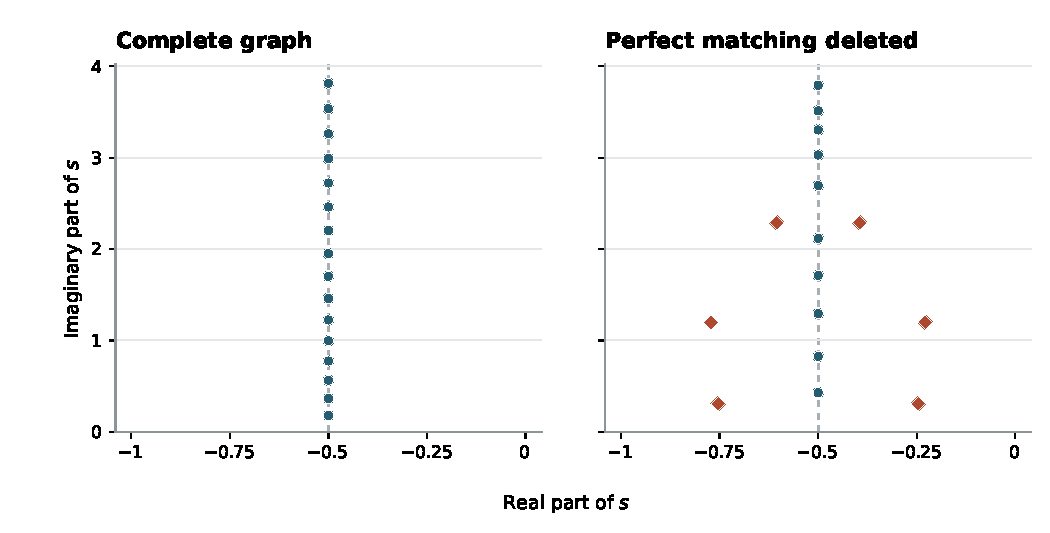
\includegraphics[width=0.9\linewidth]{roots.pdf}
\caption{Numerically located Ehrhart zeros at heights $0<\Im s<4$
in dimension $1023$. The two graphs are $K_{1024}$ and the graph obtained
by deleting a perfect matching. Diamonds mark the six off-line zeros
located in the latter plot. The data illustrate finite-dimensional
displacement. Theorems~\ref{thm:strings} and~\ref{thm:critical}
give the asymptotic conclusions.}
\label{fig:zeros}
\end{figure}

\section{Balancing parts and zeros of the Ehrhart numerator}
\label{sec:numerator}

\begin{proposition}[Schur concavity]\label{prop:schur}
At fixed vertex count $v$, moving a vertex from a larger part to a
smaller one to make the sizes more equal weakly increases every
$\gamma_j$. Equivalently, the gamma coefficients are Schur-concave in
the partition of $v$, with zero parts allowed for comparison.
\end{proposition}
\begin{proof}
Fix $j\ge1$ and put $d=v-1$. In \eqref{eq:multipartite-gamma} the loss
for one part of size $a$ is
$F(a)=\sum_{\ell>j}\binom a\ell\binom{d-a}{2j-\ell}$.
Adding one vertex to the marked part newly disqualifies precisely the
sets containing this vertex, $j$ old marked vertices and $j-1$ old
unmarked vertices. Thus
\[
 D(a):=F(a+1)-F(a)=\binom a j\binom{d-a-1}{j-1}
 \qquad(0\le a<d).
\]
Each factor is log-concave in $a$ with interval support, so their
product is unimodal. Consider the inverse move $(a,b)\mapsto(a+1,b-1)$
for $a\ge b\ge1$, with both graphs connected. Set $u=b-1$, so
$u\le a\le d-u$ and $a<d$. If $D(u)>0$, then $u>0$ and
$D(d-u)/D(u)=(d-u)/u\ge1$. Unimodality on $[u,d-u]$ gives
$D(a)\ge D(u)$. The inequality also holds when $D(u)=0$. Hence the
loss increases by $D(a)-D(u)\ge0$. Such unit transfers generate
majorization of integer partitions, and $\gamma_0=1$ throughout.
\end{proof}

Deleting $M$ disjoint edges from $K_{d+1}$ gives $M$ parts of size two,
the remaining parts being singletons. Formula~\eqref{eq:multipartite-gamma}
specializes to the gamma polynomial
\begin{equation}\label{eq:gamma-match}
 \Gamma_{d,M}(z)=G_d(z)-2Mz,\qquad
 G_d(z)=\sum_{j=0}^{\lfloor d/2\rfloor}\binom{2j}{j}\binom d{2j}z^j .
\end{equation}
The real-rootedness of $h^*$ for every complete bipartite symmetric edge
polytope~\cite[Thm.~4.8]{hjm} therefore raises a different question from
the location of the roots of $E_G$ itself.

\begin{theorem}[Threshold for real roots of the numerator]\label{thm:nonnumerator}
Write $N_d$ for the number of nonreal roots of $\Gamma_{d,M}$ with
multiplicity. The number for $h^*$ is exactly $2N_d$. Set
\[
 A_0(t)=\frac{e^{2t}}{2\sqrt\pi\,t^{5/4}},\qquad
 c_{\rm num} = A_0(5/8)=\frac{e^{5/4}}{2\sqrt\pi}(8/5)^{5/4}.
\]
\begin{enumerate}
\item For $d\ge4$ there is a real threshold $T_d$ with
$T_d/d^{3/4}\to c_{\rm num}$, such that $N_d=0$ if and only if $M\le T_d$.
\item If $M/d^{3/4}\to c>c_{\rm num}$, let $t_-<t_+$ solve $A_0(t)=c$.
Then $N_d/\sqrt d\to 2(\sqrt{t_+}-\sqrt{t_-})/\pi$.
At $c=c_{\rm num}$, $N_d=o(\sqrt d)$.
\item If $M/d^\alpha\to\lambda>0$ with $3/4<\alpha\le1$, subject to
$2M\le d+1$, then
\[
 \frac{N_d}{\sqrt{d\log d}}\ \longrightarrow\ 
 \frac{2}{\pi}\sqrt{\frac{\alpha-3/4}{2}} .
\]
In particular, a maximum matching gives
$(\sqrt2/\pi+o(1))\sqrt{d\log d}$ nonreal roots of $h^*$.
\end{enumerate}
\end{theorem}

\begin{proof}
Put $P(x)=G_d(-x)$ and $m=\lfloor d/2\rfloor$.
Let $L_d$ denote the Legendre polynomial normalized by $L_d(1)=1$.
Summing the binomial series in \eqref{eq:gamma-match} over $d$ gives
$\sum_d P(x)z^d=(1-2z+(1+4x)z^2)^{-1/2}$.
The Legendre generating function therefore gives
\[
 P(x)=(1+4x)^{d/2} L_d(\cos\theta),\qquad
 \theta=\arctan(2\sqrt{x}),\qquad x>0 .
\]
In particular $P$ has $m$ distinct positive roots, from the positive
zeros of $L_d$. We use the usual Legendre identities, orthogonality and
normalization~\cite[Ch.~18]{dlmf}.

\emph{Counting horizontal intersections.}
The negative roots of $\Gamma_{d,M}$ correspond to the positive
solutions of $Y(x)=M$, where $Y(x)=-P(x)/(2x)$. Its critical points
are given by $xP'(x)-P(x)=0$. This polynomial has at least one
zero in every gap between consecutive positive roots of $P$, by Rolle
applied to $Y$. It also has exactly one negative zero, since its value
at $x=-z$, $z>0$, is $-1+\sum_{j\ge2}(j-1)
\binom{2j}{j}\binom d{2j}z^j$. Its degree $m$ accounts for all
these zeros, each simple. Thus a bounded positive lobe of $Y$ between
consecutive zeros has one maximum. At $M>0$ it contributes two
solutions with multiplicity precisely when this maximum is at least $M$.
The first and last exterior intervals are monotone, and any positive
terminal branch attains every positive level once.
All gamma coefficients are nonnegative by Theorem~\ref{thm:gamma}, so
$\Gamma_{d,M}$ has no nonnegative real root. It follows that $N_d$ is
twice the number of positive bounded lobes whose maxima are below $M$.
For $m\ge2$ such positive lobes exist, and $T_d$ is the smallest of
their maxima. At $M=0$ all roots are real as well. Each nonreal root
$z$ of the gamma polynomial produces two distinct nonreal roots of
$z(1+t)^2=t$ in $h^*$. Each real gamma root is negative and gives
two real solutions. Any additional numerator zeros are at $t=-1$.

\emph{Legendre amplitude.}
Set $n=d+\tfrac12$, $u(\theta)=\sqrt{\sin\theta}\,L_d(\cos\theta)$,
and $q=n^2+1/(4\sin^2\theta)$. The Legendre equation gives
$u''+q u=0$. On $(0,\pi/2)$, $q$ decreases, so for
$S=u^2+u'^2/q$ we have $S'=-q'u'^2/q^2\ge0$ and $(qS)'=q'u^2\le0$.
Consequently
\[
 \frac{q(\pi/2)}{q(\theta)}S(\pi/2)\le S(\theta)\le S(\pi/2),
 \qquad S(\pi/2)\sim\frac{2}{\pi d}.
\]
The last estimate follows from
$L_{2h}(0)=(-1)^h\binom{2h}{h}/4^h$, $L_{2h+1}(0)=0$,
$L_{2h+1}'(0)=(2h+1)L_{2h}(0)$ and Stirling's formula.
Write $t=dx$ and
\[
 V_d(t)=\frac{(1+4t/d)^{d/2+1/4}}{2\sqrt\pi\,t^{5/4}} .
\]
The upper energy inequality gives
$|Y(x)|/d^{3/4}\le (1+o(1))V_d(t)$, with the prefactor uniform
in $x>0$. In each bounded lobe choose a point where $u'=0$, possible
by Rolle. At this point the lower bound is
$(1+o(1))V_d(t)\sqrt{q(\pi/2)/q(\theta)}$.
The square root is bounded below by an absolute positive constant
throughout every such lobe. Indeed, $|L_d|\le1$ on $[-1,1]$, so
Markov's polynomial inequality gives $|L_d'|\le d^2$ there, and
$L_d(\cos\theta)>0$ for $0<\theta\le1/d$. The square root converges to
one uniformly when $t$ ranges over a compact subinterval of $(0,\infty)$.

\emph{Counting lobes.}
Write $u=r\sin\psi$, $u'=nr\cos\psi$, with continuous phase and $r>0$.
The differential equation gives
$\psi'=n+\sin^2\psi/(4n\sin^2\theta)$. On any subinterval of
$[1/d,\pi/2]$ the integral of the second term is $O(1)$, by integrating
$\csc^2\theta/(4n)$. Thus the number of all zero gaps in
$[\theta_1,\theta_2]\subseteq[1/d,\pi/2]$ is
$n(\theta_2-\theta_1)/\pi+O(1)$, with half as many positive lobes up
to $O(1)$. The same estimate counts lobes meeting the interval instead
of those contained in it. Each angle gap has length at most $\pi/n$.

On a compact $t$-interval bounded away from zero the gap widths in $t$
therefore tend uniformly to zero, and $V_d(t)\to A_0(t)$ uniformly.
The maximum of each positive lobe, divided by $d^{3/4}$, is consequently
$A_0(t)+o(1)$ uniformly for any $t$ in it. For a sequence of chosen
extrema of $u$ with $t\to0$ or $t\to\infty$, the lower bound for the
normalized lobe maximum diverges. At zero this follows from $t^{-5/4}$.
At infinity, $V_d$ increases past $t=5d/(8d-16)$ and
$A_0(T)\to\infty$ as fixed $T\to\infty$. There are lobes arbitrarily
close to $t=5/8$, the unique minimum of $A_0$. These facts prove (1).

For (2), away from small neighborhoods of $t_-$ and $t_+$, the lobes
with maxima below $M$ are precisely those in $(t_-,t_+)$ for large $d$.
In a fixed $t$-interval $[a,b]\subset(0,\infty)$,
$n(\theta_b-\theta_a)/\pi=(2/\pi)(\sqrt b-\sqrt a)\sqrt d+o(\sqrt d)$.
Halving this count to take positive lobes and doubling for nonreal
roots proves (2), by shrinking the endpoint neighborhoods. For $c=c_{\rm num}$
only an arbitrarily small neighborhood of the minimum can contribute.

For (3) put $k_0=(\alpha-3/4)/2$. For any fixed $0<k<k_0$, throughout
$1\le t\le k\log d$ the upper bound $V_d(t)=O(d^{2k})$ shows that
every positive lobe contained there has maximum below $M$. For any
fixed $k>k_0$, the value
$V_d(k\log d)=d^{2k+o(1)}$ and the monotonicity of $V_d$ show that
every positive lobe whose chosen extremum is above $k\log d$ has
maximum greater than $M$. The angle at $t=k\log d$ is
$(2+o(1))\sqrt{k\log d/d}$, while the angle at $t=1$ is $O(d^{-1/2})$.
Apply the gap count to these upper and lower bounds and let $k\to k_0$.
\end{proof}

Within the family of complete graphs with a matching deleted, $d=169$
is the first dimension in which the numerator can have a nonreal
zero. For $3\le d\le168$ the program \texttt{matching\_threshold.py}
exhibits $\lfloor d/2\rfloor$ disjoint positive intervals with
alternating endpoint signs for $\Gamma_{d,M}(-x)$ at the maximum allowed
matching size. It uses trigonometric estimates only to suggest rational
endpoints; their ordering and the signs are tested by integer arithmetic.
The lobe comparison above covers all smaller matchings when $d\ge4$.
Dimensions $d\le3$ have gamma degree at most one. Across the smaller
dimensions and the check at $(d,M)=(169,84)$ there are 7,139 disjoint
root enclosures, counted within their respective polynomials.

At $d=169$ the last admissible deletion is decisive. A matching of $84$
edges gives $84$ real gamma roots and no nonreal roots. Adding the
$85$th edge to the matching leaves $82$ real roots and produces one
nonreal conjugate pair, hence four nonreal $h^*$-roots. The program
\texttt{numerator\_check.py} uses primitive signed Euclidean
remainders. Its Sturm variations at $-\infty,+\infty$ are $(84,0)$
and $(83,1)$, respectively, and both terminal remainders are nonzero
constants. An even shorter certificate suffices to show failure of
real-rootedness at $M=85$. For $P=\Gamma_{169,85}$ and
$x=-1/218$, exact rational arithmetic gives
\[
 -13348 < P'(x)^2-P(x)P''(x) < -13347.
\]
A real polynomial with only real roots satisfies
$(P')^2-PP''\ge0$ on $\mathbb R$, by differentiating its logarithmic
derivative away from the roots and extending by continuity. The checker evaluates $P,P',P''$ together by Horner's recurrence in
exact rational arithmetic.


\section{Verification and further questions}
The uniform interlacing theorem has an exact computational component.
Its certificate tests polynomial identities, integer differences, and
signs of univariate rational polynomials. These imply the assertions
for every positive integer $n$. The other principal results have
analytic or combinatorial proofs. The archive includes the exact
verifiers, their output, and the data and plotting script for
Figure~\ref{fig:zeros}.
Independent edge-step enumeration gave 312 lattice counts on 58
multipartitions through eight vertices. All 7,313 connected
multipartitions on two through 24 vertices passed degree, positivity,
and reconstruction checks. The matching identity passed 2,376 separate
evaluations. For Davis's twelve-vertex graph an exact Sturm calculation
gave seven zeros on the canonical line and four off it. These finite
checks supplement the general arguments. The new theorems are presented
as mathematical proofs with reproducible certificates. No Lean
formalization of this manuscript was performed.

Three questions follow directly. Does K\"olbl's strict interlacing hold
for all $k$ when $n$ is arbitrary? Can the quartic near a multiple
root be expanded to classify the equality case, including the effect
of rounding the matching size to an integer? Finally, does a comparably explicit threshold for numerator zeros exist
when the deleted edges form disjoint triangles or larger cliques? The
matching case in Theorem~\ref{thm:nonnumerator} depends on the loss
being linear in the gamma polynomial.

\small\begin{thebibliography}{10}\setlength{\itemsep}{3pt}
\bibitem{repo} V. Reshetnikov, \emph{ProveIt}, Analysis/GeneralizedRiemannHypothesis,
snapshot \texttt{641cd6296144} (27 November 2026). In particular
\href{https://github.com/VladimirReshetnikov/ProveIt/blob/641cd6296144d7c29bcc6569655b473647428b1b/Analysis/GeneralizedRiemannHypothesis/Article/sections/gra.tex}{Article, graph towers and Ehrhart polynomials},
subsection \emph{A bipartite family with all zeros on the canonical line}.
The project pins the upstream Dirichlet GRH development at
\href{https://github.com/lsernau/grh-lean/tree/72fead102f663d5c7a407964a13dc0cf9d977207}{\texttt{72fead102f66}}.
\bibitem{hkm} A. Higashitani, M. Kummer and M. Micha\l ek,
\emph{Interlacing Ehrhart polynomials of reflexive polytopes},
Selecta Math. (N.S.) 23 (2017), 2977--2998.
\href{https://arxiv.org/abs/1612.07538}{arXiv:1612.07538}.
\bibitem{hjm} A. Higashitani, K. Jochemko and M. Micha\l ek,
\emph{Arithmetic aspects of symmetric edge polytopes}, Mathematika 65
(2019), 763--784.
\href{https://doi.org/10.1112/S0025579319000147}{doi:10.1112/S0025579319000147}.
\bibitem{kolbl} M. K\"olbl, \emph{On a conjecture concerning the roots of
Ehrhart polynomials of symmetric edge polytopes from complete multipartite
graphs} (2024). \href{https://arxiv.org/abs/2404.02136}{arXiv:2404.02136},
in particular Theorem 3.3, Proposition 4.3 and Conjecture 4.8.
\bibitem{ot} H. Ohsugi and A. Tsuchiya, \emph{Symmetric edge polytopes
and matching generating polynomials}.
\href{https://arxiv.org/abs/2008.08621}{arXiv:2008.08621}, Theorem 3.1
and Proposition 4.1.
\bibitem{davis} C. Davis, \emph{Higashitani--Kummer--Micha\l ek conjecture},
six-pair counterexample and exact verification,
\href{https://itsdavis.com/solved-conjectures/results/hkm-ehrhart/}{itsdavis.com, result and proof record}.
\bibitem{ferroni} L. Ferroni, \emph{Symmetric edge polytopes are not
gamma-positive} (2026).
\href{https://arxiv.org/abs/2607.02424}{arXiv:2607.02424}.
\bibitem{fs} P. Flajolet and R. Sedgewick, \emph{Analytic Combinatorics},
Cambridge University Press, 2009, Ch.~VI.
\href{https://ac.cs.princeton.edu/home/}{Authors' book site}.
\bibitem{dlmf} NIST, \emph{Digital Library of Mathematical Functions},
\href{https://dlmf.nist.gov/15.8.E4}{Eq.~15.8.4} and
\href{https://dlmf.nist.gov/18}{Ch.~18, orthogonal polynomials}.
\end{thebibliography}
\end{document}
